\documentclass[a4paper,12pt]{article}
\usepackage[utf8]{inputenc}

% Variables
%Variablen welche innerhalb der gesamten Arbeit zur Verfügung stehen sollen
\newcommand{\titleDocument}{Bachelor Thesis}
\newcommand{\subjectDocument}{in Computational Linguistics}


% Embed PNG graphics
\usepackage{graphicx}
% English syllabification
\usepackage[english]{babel}
% West European encoding
\usepackage[T1]{fontenc}
% Smoother font
\usepackage{lmodern}
% Enable floating picture environments
%\usepackage{floatflt}
% Enable multi-page tables
\usepackage{longtable}
% Pretty state of the art tables
\usepackage{tabularx,booktabs}
\newcolumntype{C}{>{\centering\arraybackslash}X} % centered version of "X" type
% Set page margins
\usepackage{geometry}
\geometry{left=3.5cm, right=2cm, top=2.5cm, bottom=2cm}
% Boxes in text
\usepackage{fancybox}
% Appropriately 'syllabify' URLs
\usepackage[hyphens,obeyspaces,spaces]{url}
% Enable colored text
\usepackage{color}
% Import math symbols -- mathtools works better for this document
%\usepackage{amssymb}
% Allow writing above/below arrows + math symbols
\usepackage{mathtools}
% Heading on each page (centered)
%\pagestyle{headings}

% Enable hyperlinked Table of Contents in the PDF
\usepackage[bookmarksnumbered,pdftitle={\titleDocument},hyperfootnotes=false]{hyperref}
% Hyperlink settings
%\hypersetup{colorlinks, citecolor=red, linkcolor=blue, urlcolor=black}
%\hypersetup{colorlinks, citecolor=black, linkcolor= black, urlcolor=black}
% Cleaner headings
\usepackage{fancyhdr}
\pagestyle{fancy}
\fancyhf{} % Clean all headings/footings.
%\fancyhead[L]{\nouppercase{\leftmark}} % Left-bound heading
\fancyhead[C]{} % Centered heading
%\fancyhead[R]{\thepage} % Right-bound heading
\renewcommand{\headrulewidth}{0.4pt} %obere Trennlinie
\setlength{\headheight}{15pt}
\fancyfoot[C]{\thepage} % Include page number
%\renewcommand{\footrulewidth}{0.4pt} % Separate line at bottom of the page, does not look good imo
% Citation form: Name (Year)
\usepackage{natbib}
% Set spacing between lines - if requested
\usepackage{setspace}
% Enable captioning non-float environments
\usepackage{capt-of}
% Enable indexing - \see, \seealso, \index...
\usepackage{makeidx}
% Create index if makeidx is enabled
\makeindex
% Enable listings for code/pseudocode
%\usepackage{listings}
%\lstset{numbers=left, numberstyle=\tiny, numbersep=5pt, keywordstyle=\color{black}\bfseries, stringstyle=\ttfamily,showstringspaces=false,basicstyle=\footnotesize,captionpos=b}
%\lstset{language=python}

% List of Abbreviations -- does not work so far
\usepackage[english]{nomencl}
\let\abbrev\nomenclature
% Create index of abbreviations
\makenomenclature
% Abkürzungsverzeichnis LiveTex Version
% Title
\renewcommand{\nomname}{List of Abbreviations}
% Space between abbreviation and explanation
\setlength{\nomlabelwidth}{.25\textwidth}
% Fill space with dots
\renewcommand{\nomlabel}[1]{#1 \dotfill}
% Space between abbreviations
\setlength{\nomitemsep}{-\parsep}
\makeglossary

% Enable linguistic glossing and more. Always load last!!!
\usepackage{gb4e}
\noautomath % gb4e redefines underscores - this suppresses the redefinition

% Suppress orphans
%\clubpenalty = 10000
% Suppress widows
%\widowpenalty = 10000
%\displaywidowpenalty = 10000

\begin{document}
% Begin with empty page for print version
\thispagestyle{empty}
\mbox{}
\newpage

% TITLE PAGE %
\thispagestyle{empty}


\begin{figure}[t]
 \centering
 \includegraphics[width=0.6\textwidth]{fig/logo1}
~~~~~~~~~~
 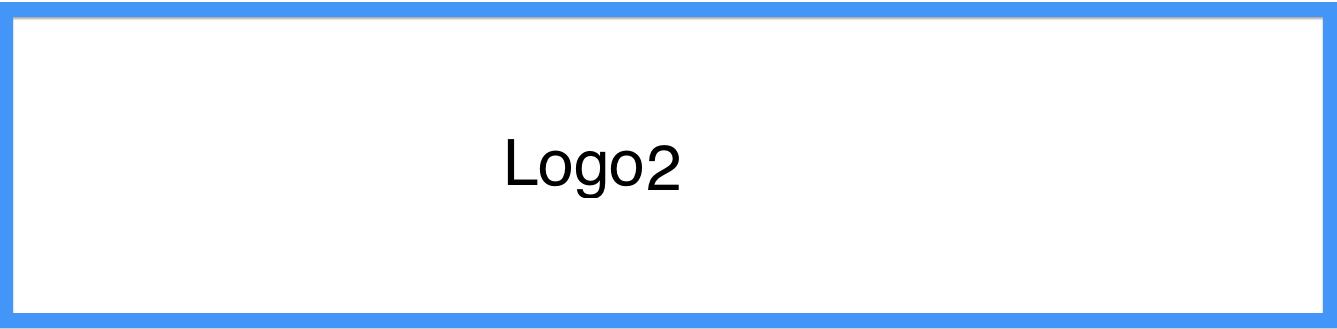
\includegraphics[width=0.3\textwidth]{fig/logo2}
\end{figure}


\begin{verbatim}


\end{verbatim}

\begin{center}
\Large{University of Potsdam}\\
%\Large{- Campus <Name> -}\\
\end{center}


\begin{center}
\Large{Faculty of Human Sciences}
\end{center}
\begin{verbatim}




\end{verbatim}
\begin{center}
\doublespacing
\textbf{\LARGE{\titleDocument}}\\
\singlespacing
\begin{verbatim}

\end{verbatim}
\textbf{{~\subjectDocument~}}
\end{center}
\begin{verbatim}

\end{verbatim}
\begin{center}

\end{center}
\begin{verbatim}

\end{verbatim}
\begin{center}
\textbf{Submitted as Partial Fulfillment of the Requirements for the Degree of \\ Bachelor of Science}
\end{center}
\begin{verbatim}






\end{verbatim}
\begin{flushleft}
\begin{tabular}{llll}
\textbf{Topic:} & & Investigating the ability of RNN architectures to learn & \\
& & context-free grammars by example of Dyck(2) & \\
& & \\
\textbf{Author:} & & Fynn Dobler <fynndobler@gmail.com>& \\
& & Matr.-Nr. 775710 & \\
& & \\
\textbf{Version of:} & & \today &\\
& & \\
\textbf{1. Supervisor:} & & Prof. Dr. Thomas Hanneforth &\\
\textbf{2. Supervisor:} & & Dr. Uladzimir Sidarenka &\\
\end{tabular}
\end{flushleft}


% 1.5x spacing for summary and abstract
\onehalfspacing
\newpage
% ABSTRACT %
\section*{Summary}

Lorem ipsum dolor sit amet, consetetur sadipscing elitr, sed diam nonumy eirmod tempor invidunt ut labore et dolore magna aliquyam erat, sed diam voluptua. At vero eos et accusam et justo duo dolores et ea rebum. Stet clita kasd gubergren, no sea takimata sanctus est Lorem ipsum dolor sit amet. Lorem ipsum dolor sit amet, consetetur sadipscing elitr, sed diam nonumy eirmod tempor invidunt ut labore et dolore magna aliquyam erat, sed diam voluptua. At vero eos et accusam et justo duo dolores et ea rebum. Stet clita kasd gubergren, no sea takimata sanctus est Lorem ipsum dolor sit amet.

\section*{Abstract}

Lorem ipsum dolor sit amet, consetetur sadipscing elitr, sed diam nonumy eirmod tempor invidunt ut labore et dolore magna aliquyam erat, sed diam voluptua. At vero eos et accusam et justo duo dolores et ea rebum. Stet clita kasd gubergren, no sea takimata sanctus est Lorem ipsum dolor sit amet. Lorem ipsum dolor sit amet, consetetur sadipscing elitr, sed diam nonumy eirmod tempor invidunt ut labore et dolore magna aliquyam erat, sed diam voluptua. At vero eos et accusam et justo duo dolores et ea rebum. Stet clita kasd gubergren, no sea takimata sanctus est Lorem ipsum dolor sit amet.


% 1x spacing for ToC
\singlespacing

% TABLE OF CONTENTS %
\newpage
\tableofcontents
% INDEX OF FIGURES - IN ToC %
\addcontentsline{toc}{section}{Index of Figures}
\listoffigures
% INDEX OF TABLES - IN ToC %
\addcontentsline{toc}{section}{Index of Tables}
\listoftables
% INDEX OF LISTINGS - IN ToC %
%\addcontentsline{toc}{section}{Index of Listings}
%\fancyhead[L]{Index of Figures/Tables/Listings}
%\renewcommand{\lstlistlistingname}{Index of Listings}
%\lstlistoflistings
% LIST OF ABBREVIATIONS - IN ToC %
\addcontentsline{toc}{section}{List of Abbreviations}
\fancyhead[L]{List of Abbreviations}
\nomenclature{RNN}{Recurrent Neural Network}
\nomenclature{MTRNN}{Multiple Timescale Recurrent Neural Network}
\nomenclature{LSTM}{Long Short-Term Memory}
\nomenclature{CFG}{Context-Free Grammar}
\nomenclature{CFL}{Context-Free Language}
\nomenclature{ANN}{Artificial Neural Network}
\printnomenclature[3cm]


%%%%%%% MAIN BODY %%%%%%%%%%%%
\newpage
\fancyhead[L]{\nouppercase{\leftmark}}
% 1,5x spacing for main work
\onehalfspacing

% einzelne Abschnitte
\section{Introduction}\label{introduction}

Lorem ipsum dolor sit amet, consetetur sadipscing elitr, sed diam nonumy eirmod tempor invidunt ut labore et dolore magna aliquyam erat, sed diam voluptua. At vero eos et accusam et justo duo dolores et ea rebum. Stet clita kasd gubergren, no sea takimata sanctus est Lorem ipsum dolor sit amet. Lorem ipsum dolor sit amet, consetetur sadipscing elitr, sed diam nonumy eirmod tempor invidunt ut labore et dolore magna aliquyam erat, sed diam voluptua. At vero eos et accusam et justo duo dolores et ea rebum. Stet clita kasd gubergren, no sea takimata sanctus est Lorem ipsum dolor sit amet.

\section{Theoretical Background}\label{theoreticalBackground}


\subsection{Formal Languages and Formal Grammars}\label{formalLanguages}
A formal language $L$ is defined as a subset of $\Sigma^{*}$ over an alphabet $\Sigma$, with $\Sigma^{*}$ being the set of all words over the alphabet. For the purpose of formal language theory, the subset of $\Sigma^{*}$ that constitutes the language $L(G)$ needs to be well-formed given the formal grammar $G$.
As per \cite{JurafskyMartin2009}, the definition of a formal grammar is $G = \lbrace N, \Sigma, R, S \rbrace$, where $N$ is a set of non-terminal symbols, $\Sigma$ is a set of terminal symbols (alphabet), $R$ is a set of rules of the form $\alpha \rightarrow \beta$ (where $\alpha$ and $\beta$ are strings of symbols from $(\Sigma \cup N)^{*}$) and $S$ is a designated start symbol.

$L(G)$ consists of all strings $w$ that can be derived from the start symbol $S$ in a finite number of steps, formally $\lbrace w \in \Sigma^{*} | S \xRightarrow [\text{G}]{\text{*}} w \rbrace$. As such, a word $w \in \Sigma^{*}$ that cannot be derived from $S$ in a finite number of steps is not part of $L(G)$.

Formal grammars differ in terms of complexity and can be described in a hierarchical manner. Grammars of higher complexity have a greater generative power than grammars of lower complexity. The most commonly used hierarchy of grammars is the Chomsky hierarchy (\cite{Chomsky1959}). In this hierarchy, formal grammars are classified into three types, sorted from most powerful to least powerful: Turing equivalent (Type 0), Context Sensitive (Type 1), Context Free (Type 2) and Regular (Type 3).

The difference in generative power and complexity stems from increasing restrictions imposed on the rules of the grammar - a Type 3 grammar is more restrictive than a Type 0 grammar. As such, every grammar of a higher type is a subset of the previous type of grammar. A visual representation of this property can be found in Figure \ref{fig:ChomskyHierarchy}.

\begin{figure}[htb]
 \centering
 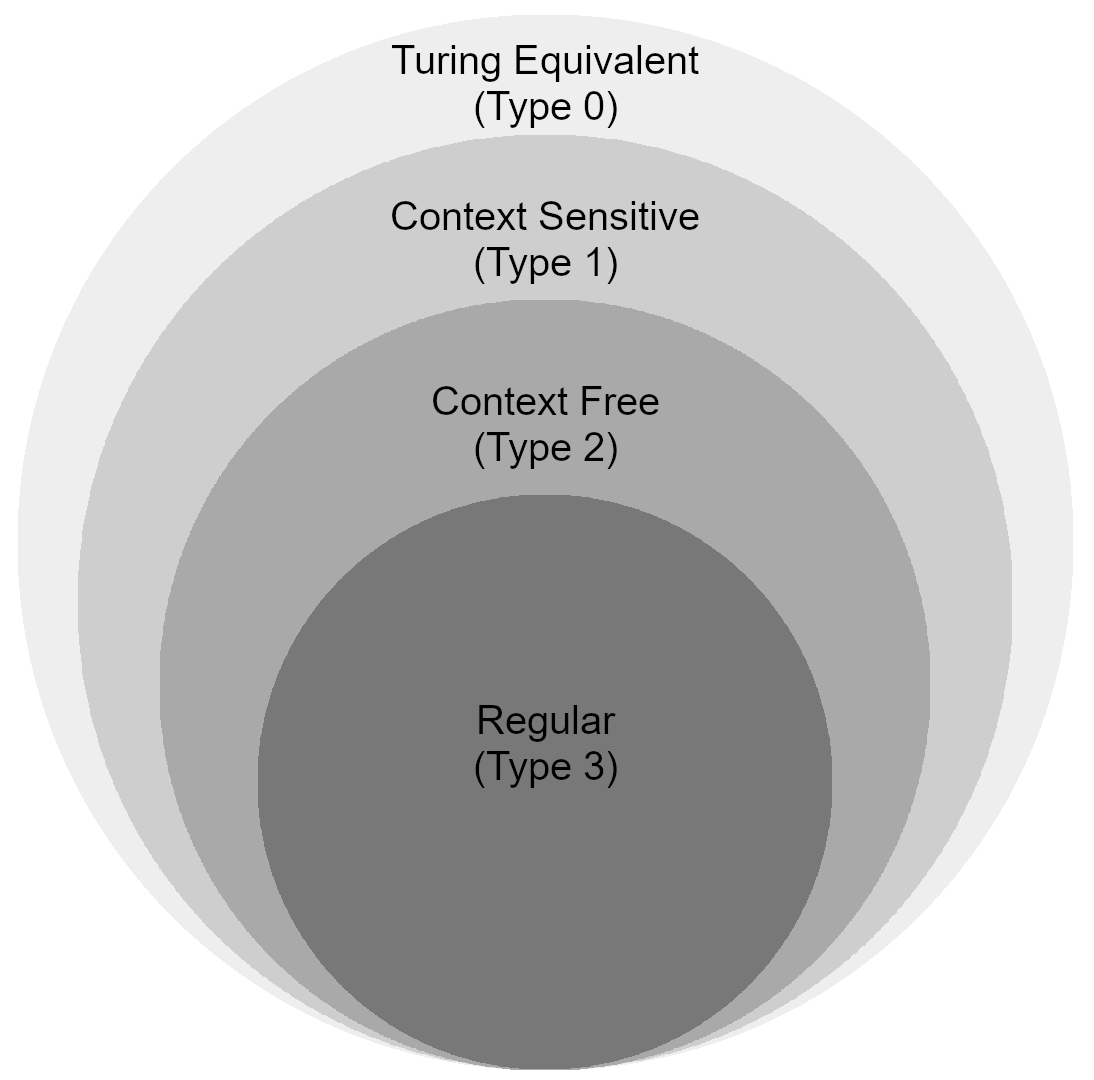
\includegraphics[width=0.5\linewidth]{fig/chomskyhierarchy}
 \caption[Chomsky Hierarchy]{A visual representation of the Chomsky Hierarchy.}
\label{fig:ChomskyHierarchy}
\end{figure}

The four types of formal grammars can be defined by the form their rules can take. An overview over these rules as per \cite{JurafskyMartin2009} can be found in Table \ref{tab:GrammarRules}, where $A$ is a single non-terminal, $\alpha$, $\beta$, $\gamma$ are strings of terminal and non-terminal symbols, and $x$ is a string of terminal symbols. $\alpha$, $\beta$ and $\gamma$ may be empty unless specifically disallowed. The table is supplemented with a column describing the corresponding automaton capable of accepting or recognizing the grammar.

\begin{table}[b]
	\begin{tabularx}{\textwidth}{@{}l*{10}{C}c@{}}
	\toprule 
	\textit{Type} & \textit{Name} & \textit{Rule Skeleton} & \textit{Automaton}\\ 
	\toprule	
	0 & Turing Equivalent & $\alpha \rightarrow \beta$, s.t. $\alpha \neq \epsilon$ & Turing Machine (recognized) \\
	1 & Context Sensitive & $\alpha A \beta \rightarrow \alpha \gamma \beta$, s.t. $\gamma \neq \epsilon$ &  Linear Bound Automata (accepted) \\
	2 & Context Free & $A \rightarrow \gamma$ & Push Down Automata (accepted) \\
	3 & Regular & $A \rightarrow xB$ or $A \rightarrow x$ & Finite-State Automata (accepted) \\
	\bottomrule	
	\end{tabularx}
	\caption[Formal grammar properties.]{Overview of formal grammar properties according to \cite{JurafskyMartin2009}, augmented with corresponding automata.}
	\label{tab:GrammarRules}
\end{table}

\subsection{Formal Grammars and Natural Language}
The correspondence of formal grammars to automata and Computational Complexity Theory lends itself to consider natural languages under the same lense. While formal grammars constitute powerful tools with which phenomena in natural language can be described, assessing precisely where natural languages lie within the Chomsky hierarchy is the subject of ongoing research.
The usual form arguments answering that question take is one of finding lower bounds: If there is a phenomenon in a natural language that cannot be described with a given grammar, natural language must be - however slighty - more complex than that type allows. Such arguments increase in credibility the more frequently they can be replicated for phenomena in multiple languages. The arguments establishing natural languages as supra-context-free (i.e. more complex than CFGs) as well as contrary evidence from empiric research shall be presented here.

\subsubsection{Natural Language as supra-regular}\label{supraReg}
English, as well as several other languages (\cite{Hagege1976}) allow for center embedding, the embedding of a phrase into another phrase of the same type.
\begin{exe}
	\ex The man eats.
	\ex The man the boss fired eats.
	\ex The man the boss the investor distrusted fired eats.
	\ex The man the boss the investor the police investigated distrusted fired eats.
\end{exe}
Let the set $E$ contain all grammatical sentences of English, and let the noun phrases and transitive verbs constitute following sets:
\begin{align*}
A &= \lbrace \text{the boss}, \, \text{the investors}, \, \text{the police}, \dots \rbrace \\
B &= \lbrace \text{fired}, \, \text{distrusted}, \, \text{investigated}, \dots \rbrace
\end{align*}
Then the following two sets can be defined.
\begin{align*}
E' &= \lbrace \text{the man } a^{n}b^{n} \text{ eats} \: \vert \: n \geq 0 \rbrace \\
R &= \lbrace \text{the man } a^{*}b^{*} \text{ eats} \rbrace
\end{align*}
$a^{n}$ and $b^{n}$ are finite sequences of size $n$ of elements of sets $A$ and $B$, respectively. $E'$ describes a subset of $E$, namely $E \cap R$. Since regular languages are closed under intersection and $E'$ is not regular, $E$ is not regular.\footnote{The proofs for regular languages being closed under intersection and $E'$ not being regular can be found in the appendix.}

While this proof is correct under the framework of Formal Language Theory, the validity of claiming that it shows natural language to be supra-regular is debatable. Research in psycholinguistics shows that native speakers have face severe problems processing center embeddings of depth two or higher, yielding long processing times, an incomplete understanding of the presented sentence or leading the participants to judge the sentence as ungrammatical (\cite{Hamilton1971}, \cite{Frank2016}). Furthermore, the corpus-driven analysis by \cite{Karlsson2007} suggests an upper limit of center embedding depth three in the seven investigated languages.

The proof concerns linguistic competence, whereas empirical studies provide an insight into linguistic performance. Usually, the distinction between competence and performance provide an adequate framework for both theoretical and empirical work, but when discussing the complexity of natural language neither side should be discarded. A linguistic competence framework cannot appropriately declare natural language as supra-regular if natural language is produced and processed according to regular rules. Conversely, for the purposes of computational linguistics, exclusively assessing linguistic performance by way of corpus analysis is insufficient, as a corpus of any size pales in comparison to the potential for infinitely many combinations that characterizes language. For the purposes of NLP, it is recommendable to err on the side of overestimating the complexity of natural language - so long as the resulting models are sufficiently efficient and accurate.

\subsubsection{Natural Language as supra-context-free}

Similarly to the proof given in Section \ref{supraReg}, an argument characterizing natural language as supra-context-free can be brought forth. It is based on embedded infinitival verb phrases found in Swiss German (\cite{Shieber1987}).
\begin{exe}
	\ex
	\gll Jan säit das mer em Hans es huus haend wele hälfe aastriiche. \\
	Jan said that we the Hans-DAT the house-ACC have wanted help paint \\
	\trans 'Jan said that we have wanted to help Hans paint the house.'
	\ex
	\gll Jan säit das mer d'chind em Hans es huus haend wele laa hälfe aastriiche. \\
	Jan said that we the children-ACC the Hans-DAT the house-ACC have wanted let help paint \\
	\trans 'Jan said that we have wanted to let the children help Hans paint the house.'
\end{exe}
Four finite sets can be constructed from these examples: accusative noun phrases ($A = \lbrace \text{d'chind}, \, \dots \rbrace$), dative noun phrases ($B = \lbrace \text{em Hans}, \, \dots \rbrace$), transitive verbs taking accusative objects ($C = \lbrace \text{laa}, \, \dots \rbrace$) and transitive verbs taking dative objects ($D = \lbrace \text{hälfe}, \, \dots \rbrace$). Let the set $S$ then be the set of all grammatical sentences of Swiss German. Again, the two following sets can be defined:
\begin{align*}
S' &= \lbrace \text{Jan säit das mer } a^{n}b^{m} \text{ es huus haend wele } c^{n}d^{m} \text{ aastriiche} \: \vert \: n, m \geq 0 \rbrace \\
R &= \lbrace \text{Jan säit das mer } a^{*}b^{*} \text{ es huus haend wele } c^{*}d^{*} \text{ aastriiche} \rbrace
\end{align*}
$S'$ is not context-free and results from $S \cap R$. Since context-free sets are closed under intersection with regular sets, $G$ cannot be not context-free.\footnote{The respective proofs for $S'$ not being context-free and context-free sets being closed under intersection with regular sets can be found in the Appendix.}

Curiously enough, empirical research into the matter of processing similar cross-serial dependencies in Dutch suggests them to be generally easier to process than nested dependencies (i.e. the ones used to prove natural language to be supra-regular) (\cite{Bach1986}).

\subsection{Dyck Languages}\label{dyckLanguages}
Whether natural language is regular, context-free, supra-regular or supra-context-free is a distinction of only tangential relevance for this work. The first two cases are fully covered by CFGs, while the other two leave room for some natural language productions outside of the scope of CFGs. The characteristics of supra-context-free examples in natural language show a \textit{weak} non-context-freeness, making CFGs sufficient for covering the vast majority of natural language productions. With this assumption, an appropriate CFG for a model to learn must be found. The most important property of this grammar is that model performance on its language must allow for strong conclusions about the learnability of any other CFG. In doing so, one can make reasoned assumptions about potential model performance on natural language data. 

One such a grammar is the Dyck Grammar, which can produce an array of Dyck Languages. Let $D_{n} = \lbrace N, \Sigma, R, S \rbrace$ with
\begin{align*}
	N &= \lbrace S \rbrace \\
	\Sigma &= \lbrace \epsilon, O_{1}, O_{2}, \dots, O_{n}, C_{1}, C_{2}, \dots, C_{n} \rbrace \\
	R &= \lbrace \\
		 & \: S \rightarrow \epsilon \\
		 & \: S \rightarrow O_{n} \, S \, C_{n} \, \rbrace ,
\end{align*}
where $O_{n}$ represents an opening parenthesis, $C_{n}$ represents a closing parenthesis and $n$ denotes the number of distinct pairs of parentheses. $D_1$, then, denotes the Dyck Language with $\Sigma = \lbrace \epsilon, (, ) \rbrace$, $D_2$ the Dyck Language with $\Sigma = \lbrace \epsilon, (, [, ], ) \rbrace$, et cetera.

Within the family of Dyck Languages, $D_2$ is of particular interest. According to the Chomsky-Schützenberger Representation Theorem \citep{Chomsky1963}, for every context-free language $L$ there exists a positive integer $n$, a regular language $R$, and a homomorphism $h$ so that $L = h(D_{n} \cap R)$. Following the proof in \cite{Autebert1997}, a homomorphism $g_{n}$ can be constructed so that $D_{n} = g_{n}^{-1}(D_{2})$. It follows that every context-free language can be represented as $L = h(g_{n}^{-1}(D_{2}) \cap R)$. As such, every CFL could be represented via homomorphisms on $D_2$ and intersections with a regular language\footnote{NDFL vs DFL!}. Assuming natural languages to be context-free and bearing in mind that using a formal language is a choice of abstraction which allows for precise control over corpus composition, this makes $D_2$ the language of choice when evaluating neural network performance on a comparative scale.
%TODO proof, basically
%TODO NDFL vs DFL footnote

\subsection{Neural Network Architectures}\label{neuralNetworkArchitectures}

\subsubsection{Simple RNN}\label{SRNN}
Recurrent Neural Networks (RNNs) (\cite{Elman1990}) are a neural network architecture particularly suited to processing sequential information by virtue of them being recurrent: the RNN's output at a time step $t$ is fed back as its input at the following time step $t+1$. As such, every output is dependent on the previous computation as well as the current input. This property equips RNNs with a "memory" with regards to previous inputs, allowing them to capture context dependencies a context agnostic model cannot adequately learn.

Within the frame of this work, the specific case of the Simple RNN (SRNN) is considered. It is a three layer networks, consisting of an input layer, a hidden layer and an output layer. The hidden state $h_t$ at time step $t$ given the input vector $x_t$ and the output vector $y_t$ are calculated as per the following equations:

\begin{align}
	h_{t} &= f(\boldsymbol{W_{xh}} x_{t} + \boldsymbol{W_{hh}} h_{t-1}) \\
	y_{t} &= \boldsymbol{W_{hy}} h_{t}
\end{align}

The function $f$ constitutes a non-linear transformation, like $\tanh$ or ReLU. $\boldsymbol{W_{xh}}$, $\boldsymbol{W_{hh}}$, $\boldsymbol{W_{yh}}$ are matrices of the weights connecting the input layer to the hidden layer, the hidden layer to itself and the hidden layer to the output layer, respectively.

When training RNNs, it is beneficial to think of the network as unfolding into an architecture with one layer per time step. A visualisation is provided in Figure \ref{fig:unrolledRNN}. As such, the RNN can be treated as a deep feedforward network. These conceptual layers share their parameters - if any weight changes at time step $t$, the weight also changes at $t+1, t+2, \dots, t+n$. Isolated changes are not possible. A popular training algorithm for RNNs is Backpropagation Through Time (BPTT) (\cite{Williams1998}), a gradient based algorithm designed for recurrent rather than feedforward networks. However, as \cite{Bengio1994} and \cite{Hochreiter1998} show, RNNs suffer from a fundamental flaw: the aptly named vanishing gradient problem, in which the training gradient diminishes to zero throughout the layers.

\begin{figure}[htb]
 \centering
 \includegraphics[width=0.6\textwidth]{fig/logo1}
 \caption[Unfolded RNN]{An RNN, unfolded through time.}
\label{fig:unrolledRNN}
\end{figure}

%TODO RNN unfold graphic (check Young et al. 2018 p.11 for an example
%TODO (maybe!) brief overview of sources utilizing RNNs for NLP and formal language eval

\subsubsection{LSTM}\label{LSTM}

Long-Short Term Memory networks (LSTM) were designed by \cite{Hochreiter1997} as an RNN architecture which preserves the RNN capabilities of processing sequential data of arbitrary length and capturing context dependencies, while circumventing the vanishing gradient problem.

LSTMs are based on self-connected linear units which are regulated by three multiplicative gates: input (in), output (out) and forget ($\varphi$). At every time step, the concatenated vector of the previous hidden state $h_{t-1}$ and the current input $x_{t}$ are received by all three gates. Given this input, the gates apply individual multiplicative factors $m_{\text{Gate}} \in [0, \dots, 1]$, determining what information is let through the input gate, passed through the output gate or forgotten by the self-connected linear unit.

\begin{align*}
\text{in}_{t} &= m_{\text{in}} (\boldsymbol{W_{\text{in}}} \cdot [h_{t-1},x_{t}] + b_{\text{in}}) \\
\text{out}_{t} &= m_{\text{out}} (\boldsymbol{W_{\text{out}}} \cdot [h_{t-1},x_{t}] + b_{\text{out}}) \\
\varphi_{t} &= m_{\varphi} (\boldsymbol{W_{\varphi}} \cdot [h_{t-1},x_{t}] + b_{\varphi})
\end{align*}

Finally, the cell state $C_{t-1}$ is updated to $C_{t}$ and $h_{t}$ is set.

\begin{align*}
C_{t} &= \text{forget}_{t} \odot C_{t-1} + \text{in}_{t} \odot \tanh (\boldsymbol{W_{C}} \cdot [h_{t-1},x_{t}] + b_{\text{C}}) \\
h_{t} &= \text{out}_{t} \odot \tanh (C_{t})
\end{align*}

\begin{figure}[htb]
 \centering
 \includegraphics[width=0.6\textwidth]{fig/logo1}
 \caption[LSTM Memory Cell]{An LSTM memory cell, bla, bla bla.}
\label{fig:memoryCellLSTM}
\end{figure}

%TODO LSTM memory cell figure (check Hochreiter 1997 or explanations for reference)
%TODO (maybe!) brief overview of sources utilizing LSTMs for NLP and formal language eval

\subsubsection{GRU}\label{GRU}
A less complex alternative to LSTMs, the Gated Recurrent Unit (GRU) was developed by \cite{Cho2014}. The information flow within the GRU is handled by just two gates: reset ($r$) and update ($z$). The update gate determines how much information from previous time steps is passed along for further time steps, while the reset gate enables the model to drop irrelevant information and only consider the current input rather than the previous hidden state, as described in the equations below, where $j$ is the $j$-th hidden unit, $\sigma$ is the squashing sigmoid function, $\boldsymbol{W}$ and $\boldsymbol{U}$ are learned gate-dependent weight matrices and $\phi$ is a non-linear function.

\begin{align*}
r_j &= \sigma \big( [\boldsymbol{W_{r}}x]_{j} + [\boldsymbol{U_{r}}h_{t-1}]_{j} \big) \\
z_j &= \sigma \big( [\boldsymbol{W_{z}}x]_{j} + [\boldsymbol{U_{z}}h_{t-1}]_{j} \big) \\
h_{j}^{t} &= z_{j}h_{j}^{t-1} + (1 - z_{j}) \tilde{h}_{j}^{t} \\
\tilde{h}_{j}^{t} &= \phi \big( [\boldsymbol{W}x]_{j} +[\boldsymbol{U}(r \odot h_{t-1}]_{j}) \big)
\end{align*}

\begin{figure}[htb]
 \centering
 \includegraphics[width=0.6\textwidth]{fig/logo1}
 \caption[Illustration of a GRU]{Illustration of a GRU.}
\label{fig:GRU}
\end{figure}

%TODO GRU figure (see Young et al. 2018 page 12/Cho et al 2014 for reference)
%TODO (maybe!) brief overview of sources utilizing GRUs for NLP and formal language eval

\subsection{Related Works}\label{relatedWorks}
%TODO This section desperately needs a rewrite. Give it an actual narrative, rather than just being a laundry list of previous papers.

Formal languages have been used to evaluate the performance of neural network architectures for decades (\cite{Cleeremans1989}, \cite{Zeng1994}, \cite{Hochreiter1997}, \cite{Rodriguez1998}, \cite{GersSchmidhuber2001}, \cite{JoulinMikolov2015}). These papers frequently determine how well the architecture can generalize from training on a relatively small subset of the language to testing on longer unseen words. (Example results)
%TODO Specific example results, i.e. "LSTMs can learn CSLs"
%TODO include research into automaton extraction from neural networks for regular and context-free grammars


While these results make for compelling cases in favour of the architectures proposed by the authors, the methodology has recently come under criticism by researchers like \cite{Bernardy2018}, \cite{Sennhauser2018}. The former goes as far as to say that none of the previous research compellingly shows RNNs to be capable of learning nested hierarchical structures.
%TODO Reread and specifically state Bernardy's criticism


Formal languages making up early performance benchmarks for neural networks was, in the early years of RNN research, at least partially caused by the lack of comparable natural language corpora and of reliable hardware with sufficient computational power. By now, of course, these restrictions are far above the levels of 1990 (Elman RNN). This lead to a sizeable corpus of research on NLP, i.e. \cite{Karpathy2015}.
%TODO more elegant mention of NLP research and NLP application


There are several recent works investigating neural architectures and their capability of learning Dyck languages specifically. [They feature a variety of ways of sampling their corpora, evaluate models on different tasks and report a varying subset of relevant performance measures.]

\cite{Deleu2016} evaluate the capability of a Neural Turing Machine (NTM) to deal with long-term dependencies. The model performs a membership classification task on words belonging to D$_1$ and non-words using the same alphabet, but not belonging to D$_1$. The NTM shows strong generalization by correctly recognizing well over $90 \%$ of D$_1$ words with length 180, despite only being trained on words of length $<12$. The authors do not report on any other measures of performance.

\cite{Li2018} deserve a mention in this section for evaluating their nonlinear weighted finite automata on a corpus generated by a probabilistic D$_1$ grammar and reporting on word error rate (WER) relative to the size of the training set. The size of the training set ranges from $200$ to $20,000$, with a fixed test set size of $250$.

\cite{Skachkova2018} compare the accuracy and perplexity of Elman-RNNs, GRUs and LSTMs learning D$_1$, D$_2$, D$_3$, D$_4$ and D$_5$. The respective corpora are generated by a probabilistic Dyck grammar, with the given rule probabilities controlling the average length of the generated sequences.

\cite{Sennhauser2018} choose an approach that demonstrates whether an LSTM can learn hierarchical structures by training the models for a prediction task on one million D$_2$ words with length 100. Their training corpus has been sampled from a probabilistic D$_2$ grammar. They report on two further corpus properties: distance, which is the number of characters between an opening bracket and its corresponding closing bracket, and embedded depth, which is the maximum number of unclosed brackets in a processed word. They report error rate, predictable distances and embedded depth in relation to number of hidden units. Furthermore, they perform an Intermediate State Analysis. Their results suggest the trained models fail at correctly learning the rules of the D$_2$ grammar.

\cite{Suzgun2019} offer an overview of small-sized Elman-RNNs, GRUs and LSTMs learning D$_1$, D$_2$ and corresponding shuffle languages. They report accuracy and provide an analysis of the LSTM cell state dynamics. They find that none of their models are capable of learning D$_2$, with the highest scoring model (LSTM) achieving a $48.24\%$ accuracy.

The topic of investigation of \cite{Yu2019} lies outside of the scope of this thesis, as it is predominantly concerned with the seq2seq framework and attention mechanisms. However, their data set consists of largely the same settings as \cite{Sennhauser2018} have used. Additionally, they report many of the same measures of performance.

An overview of investigated Dyck languages, corpus sizes and reported measures of performance can be found in Tables \ref{tab:LiteratureCorpusOverview}, \ref{tab:LiteratureInvestigatedModels} and \ref{tab:LiteratureReportedMeasures}.

\begin{table}
	\begin{tabularx}{\textwidth}{@{}l*{10}{C}c@{}}
		\toprule 		
		\textit{Paper} & \textit{D$_n$} & \textit{Grammar Probability} & \textit{Training Corpus Size} \\ 
		\toprule 
		\cite{Deleu2016} & 1 & equal & unclear \\ 
		\cite{Li2018} & 1 & modified & $200$ - $20,000$ \\ 
		\cite{Skachkova2018} & 1-5 & modified & $131,072$ \\ 
		\cite{Sennhauser2018} & 2 & modified & $1,000,000$ \\ 
		\cite{Suzgun2019} & 1-2 & modified & $10,000$ \\ 
		\cite{Yu2019} & 2 & modified & $1,000,000$ \\ 
		\bottomrule
	\end{tabularx}
	\caption[Corpus sizes in current works]{Overview of corpus sizes in current works.}
	\label{tab:LiteratureCorpusOverview}
\end{table}


\begin{table}
	\begin{tabularx}{\textwidth}{@{}l*{10}{C}c@{}}
	\toprule 
	\textit{Paper} & \textit{Architectures}\\
	\toprule 
	\cite{Deleu2016} & Neural Turing Machine, LSTM\\
	\cite{Skachkova2018} & Elman-RNN, GRU, LSTM\\
	\cite{Sennhauser2018} & LSTM\\
	\cite{Suzgun2019} & Elman-RNN, GRU, LSTM\\
	\cite{Yu2019} & seq2seq\\ 
	\bottomrule
	\end{tabularx}
	\caption[Overview of investigated models]{Overview of investigated models.}
	\label{tab:LiteratureInvestigatedModels}
\end{table} 

% Can be put into appendix with [p] option
\begin{table}
	\begin{tabularx}{\textwidth}{@{}l*{10}{C}c@{}}
	\toprule 
	\textit{Paper} & \textit{Accuracy} & \textit{Perplexity} & \textit{Cell State} & \textit{AUC} & \textit{Error Rate} \\
	\toprule
	\cite{Deleu2016} & No & No & No & Yes & No \\
	\cite{Skachkova2018} & Yes & Yes & No & No & No \\
	\cite{Sennhauser2018} & No & No & Yes & No & Yes \\
	\cite{Suzgun2019} & Yes & No & Yes & No & No\\
	\cite{Yu2019} & No & Yes & No & No & Yes \\ 
	\bottomrule
	\end{tabularx} 
	\caption[Reported values for performance in previous works]{Overview of reported values for performance. Cell State Analysis does not refer to a unified method, it merely means the paper investigates cell states at all. AUC refers to the area under the curve for an increasing length of Dyck words the model was able to generalize.}
	\label{tab:LiteratureReportedMeasures}
\end{table} 

In conclusion, there is currently no benchmark Dyck corpus within the literature upon which to evaluate model performance. Furthermore, there is also no consensus on which measures of performance to report. Considering how wildly the corpora and the reported measures of performance differ, the results of the publications mentioned here cannot be directly compared with each other. This allows for no conclusive statement on the relative performance of various popular RNN architectures based on the current literature.
\section{Experiment Setup}\label{experimentSetup}

\subsection{Models}\label{models}
For the following experiments, the three RNN architectures described in Section \ref{neuralNetworkArchitectures} have been used. All models consist of a single layer of size $n = \lbrace 2^{1}, 2^{2}, \dots, 2^{n} \rbrace$, followed by a dense layer of size 5 with softmax activation. Each neuron in the dense layer corresponds to one character in the training data - \texttt{\{}, \texttt{[}, \texttt{]}, \texttt{\}} and \$ as an end-of-word marker. As such, the activations of the dense layer serve as interpretable output.

All models were trained with the same parameters. The training data was received one character at a time, in batches of $512$. The loss was computed by categorical cross-entropy. Furthermore, the Adam optimizer (\cite{Kingma2014}) was applied with a learning rate of $0.0001$. The models were trained for $50$ epochs each. From those $50$ epochs, the model with the lowest loss was chosen to perform on the test data.\footnote{The models were implemented in Tensorflow 2.0. The source code can be found at URL HERE} %TODO

The models were trained on the same training data for both experiments. To answer the question of training data influence on model performance, three distinct sets of training data were used, yielding a total of $9 \times 3 \times 3 = 81$ evaluated models.

\subsection{Corpus Construction}\label{corpusConstruction}
To investigate the influence of corpus composition on model performance, three corpora were created: a baseline corpus which is directly sampled from a subset of $D_{2}$, as well as two modifications of the baseline corpus: one impoverishing the training data from long-range dependencies (Low LRD) and one enriching the training data with more long-range dependencies (High LRD). The sampling and modification processes will be explained later in this section.

The experiments were explicitly designed to test the models' abilities to generalize based on the training data they encounter. As such, it is prudent to give consideration to which properties the training data might possess to facilitate or inhibit generalizability - properties such as length, nesting depth (ND) and the distance between a pair of opening and closing brackets (BD). These measures are in terms of averages and variance in Table \ref{tab:Corpora}.

\begin{table}
	\begin{tabularx}{\textwidth}{@{}l*{10}{C}c@{}}
		\toprule 		
		\textit{Corpus} & \textit{Word Length} & \textit{maxND} & \textit{maxBD} \\ 
		\toprule 
		Baseline & 18.38 & 4.31 & 13.03 \\
		Low LRD & BLA & BLA & BLA \\
		Low LRD & BLA & BLA & BLA \\
		\bottomrule
	\end{tabularx}
	\caption[Training corpora properties]{Properties of the three corpora the models were trained on.}
	\label{tab:Corpora}
\end{table}

Furthermore, the training corpora were chosen to be a small slice of a comparatively large subset of $D_{2}$. To facilitate generalization, the training corpora consist of words of varying length. As discussed in Section \ref{relatedWorks}, previous works largely utilized similarly small language subsets and achieved encouraging results. For a discussion of Experiment $1$ and $2$ on a training corpus consisting of a majority of the target language, see \cite{Bernardy2018}.

In determining an eligible maximum length, a fact about the size of $D_{n}$ subsets ways used: a Dyck language $D_{n}$ contains $n^mC_{n}$ words of length $2m$, where $C_{m}$ is the $m$-th Catalan number (\cite{Skachkova2018}). It follows that a maximum length limit of $2m$ produces a set of size $\sum_{i=2}^{2m}n^{i}C_{i}$. For example, a maximum length of 20 in $D_{2}$ ($D_{2}^{\leq 20}$) yields $20,119,506$ words, which is a sufficiently large subset to sample from. The words were generated following the probabilistic grammar set forth by \cite{Sennhauser2018}.
\begin{align*}
	S &\rightarrow Z \; S \; \vert \; Z \\
	Z &\rightarrow B \; \vert \; T \\
	B &\rightarrow [ \; S \; ] \; \vert \; \lbrace \; S \; \rbrace \\
	T &\rightarrow [ \; ] \; \vert \; \lbrace \; \rbrace
\end{align*}

The production $Z \rightarrow B$ branches, whereas $S \rightarrow Z \; S$ concatenates two smaller Dyck words. This representation provides a good intuition for understanding the merit of Experiment 1. The probabilities with which the rules were applied are calculated as follows, with alternative rules of course being applied with the complementary probability:
\begin{align*}
	P_{\text{branch}} &= r_{\text{branch}} \cdot s(l) \quad \text{with } r_{\text{branch}} \sim U(0.7,1.0) \\
	P_{\text{concat}} &= r_{\text{concat}} \cdot s(l) \quad \text{with } r_{\text{concat}} \sim U(0.7,1.0) \\
	s(l) &= \min(1, -3 \cdot \frac{l}{n} + 3)
\end{align*}
with $l$ being the number of already generated non-terminal characters and $n$ the maximally desired length of the word. $r_{\text{branch}}$, $r_{\text{concat}}$ and $l$ were sampled at every step of word generation.

Following this process, $140,000$ words in $D_{2}^{\leq 20}$ were generated. These words served as the basis for creating the three corpora. To created the Low LRD corpus, all words with a maximum bracket distance higher than $14$ were modified\footnote{This cutoff point was chosen as it significantly reduces the average maximum bracket distance without creating too many duplicates.} by first identifying the bracket pair with the highest bracket distance, then simply moving the opening bracket from its original position to the position right before the closing bracket. (i.e. \texttt{\{[\{\}]\}} becomes \texttt{[\{\}]\{\}}). This has the largest impact on bracket distance throughout the corpus, while ensuring grammaticality of the resulting word. The resulting set of long-range impoverished words was merged with all unmodified words, deleting all duplicates.

The High LRD corpus was created in a similar way: First, all words with a bracket distance lower than 18 were identified.\footnote{The same considerations as for the Low LRD corpus cutoff apply.} Then, the first pair of neighboring closing brackets is found and deleted. The remaining word is wrapped in a randomly chosen pair of brackets, creating the longest possible bracket distance between the two (i.e. \texttt{\{[\{\}]\}} becomes \texttt{\{\{[]\}\}}). The resulting set was merged with the unmodified words the same way as the Low LRD set.

The deletion of duplicates naturally leads to not all $140,000$ initially created words being used for training. Indeed, the chosen cutoff points resulted in a much smaller Low LRD set of $87,311$ words. For the sake of keeping training in full batches of $512$, the closest multiple of the batch size is $512 \times 170 = 87,040$, leading to a training corpus size of $512 \times 170$ words. Furthermore, since the investigated manipulations were the changes in ND and BD and not the effects of corpus size, the Baseline and High LRD corpus were truncated to size $512 \times 170$ by randomly removing surplus words.

\subsection{Evaluation}\label{evaluation}
The designs for the first two experiments closely follow the procedure described by \cite{Bernardy2018} - and the evaluation procedure was inspired by the discussion in his work as well. As he notes, it is indeed impossible to achieve a full $100\%$ accuracy on prediction tasks for Dyck languages. This is owed to the fact that at any position within a word, the valid options for the next character encompasses all opening brackets in addition to whichever closing bracket might be appropriate (i.e. the sequence \texttt{[[\{\}]} can be followed by either \texttt{]}, \texttt{\{} or \texttt{[}). Indeed, this makes deciding how to score accuracy for the following experiments rather difficult. Obviously, an assessment of accuracy only ever makes sense when the next character in the test word is a closing bracket - when there is no prescribed limit to the length of a Dyck word, opening brackets are never a wrong prediction. But how to score accuracy on the position of the closing bracket? Either, one only assesses the correct closing bracket as the one correct prediction, or one allows all predictions except the wrong closing bracket and the end-of-word marker to be seen as correct.

In a series of experiments designed to assess how well - if at all - neural network models can learn the underlying grammar of a training corpus, choosing the first option seems counterintuitive. After all, predictiong an opening bracket instead of the expected closing bracket could be an indication for appropriate rule application. However, accepting all open bracket predictions to be correct does not contribute to an accurate assessment of grammaticality either: Once the model has predicted an opening bracket in place of a closing bracket, it is assuming a structurally very different word than is actually present in the test set. This predicted word would have a deeper nesting depth and a longer-running range dependency than the test word. A much more insightful measure, then, is to ask whether the model actually closes its predicted opening bracket.
% Alternatively: Looking at the Dense layer output by index for both experiments to evaluate the development of opening + correct closing bracket activations. Expected: Opening bracket activation declines with increasing word length. Ideal: Close-to-equal activation for all opening + proper closing bracket, very low activation for improper closing bracket.

Since there is no elegant way to unite both approaches, the idea of assessing a model's capability of closing a self-predicted bracket will be pursued in Experiment 3. For Experiments 1 and 2, accuracy will be calculated more strictly. If, and only if the next character in the test word is a closing bracket will the model's prediction be evaluated. If the model predicted the correct closing bracket, it has made a correct prediction. Every other prediction is rated as false. As such, the model accuracy by character index is calculated as follows:
\[
	\text{acc}_{i} = \frac{\text{\# of correct predictions up to index }i}{\text{\# of closing brackets up to index }i}
\]
A random guessing strategy choosing from all brackets in the alphabet yields a baseline $25\%$ acuracy. A perfect predictor, then, could score $100\%$ if it both perfectly resulves all opening and closing bracket dependencies and never predicts an open bracket instead of a closed one.
%Bold claim: This indeed would make a 100% accuracy both undesireable and puzzling - and an indication that the model has not actually learned a generalizable grammar resembling D_{2}. In reality, a prefect predictor that has learn D_{2} should score around $33,33\%$ accuracy. The remaining $66,66\%$ are split equally on the two opening brackets.

\subsubsection{Experiment 1: Long-Range Dependency}\label{LRD}
For this experiment, the test set consisted of $512 \times 17$ Dyck words with length $1+18+18+1=38$. They were created by picking two random Dyck words $w_{1}, w_{2} \in D_{2}^{=18}$ from the previously generated $140,000$ words $\in D_{2}^{\leq 20}$, concatenating them and wrapping the result in a randomly selected pair of matching brackets as follows:
\[
	w_{\text{LRD}} = O_{n}w_{1}w_{2}C_{n}
\]
While $w_{1}$ and $w_{2}$ might have been seen in training, the resulting word most certainly has not been observed. Neither could the model possibly have encountered a long-range dependency spanning $36$ characters between the opening and closing bracket. As such, a high accuracy on the final character of the word serves as a strong indication for the model having not just learned the necessity of closing open brackets to form an acceptable Dyck word, but also for the model having retained information on the first opening bracket during all processing steps. For further insight in model behaviour, the accuracy is reported for every processed character.

\subsubsection{Experiment 2: Deeper Nesting}\label{DN}
To investigate how well a model performs on predicting brackets on a nesting level deeper than anything included in training, another test set was constructed. Generalizing to extreme long-range dependencies as in Experiment 1 is not necessary for this task, leading to the words being significantly shorter.

For this task, $512 \times 17$ words $w \in D_{2}^{=20}$ have been chosen at random. They were then wrapped by a prefix of five randomly chosen opening brackets and a suffix of the corresponding closing brackets as follows:
\[
	w_{\text{DN}} = O_{n}O_{n}O_{n}O_{n}O_{n}wC_{n}C_{n}C_{n}C_{n}C_{n}
\]
This process still has the model extrapolate beyond the length of the training words, while not confounding the results with LRD performance too much. Indeed, when analysing the results, the main focus lies on the infixed word, since all its nesting depths are now increased by 5, possibly affecting model performance.

\subsubsection{Experiment 3: Generating Depth}\label{GD}
\section{Results}\label{results}
\section{Discussion}\label{discussion}
\section{Conclusion}\label{conclusion}

% 1x spacing for Bibliography
\singlespacing

\newpage
% Bibliography appears in ToC
\addcontentsline{toc}{section}{Bibliography}
\renewcommand\refname{Bibliography}
\bibliography{master}
\bibliographystyle{myapalike}


\onehalfspacing
% APPENDIX %
\newpage
% Appendix appears in ToC
\addcontentsline{toc}{section}{Appendix}
\fancyhead[L]{Appendix}
\subsection*{Appendix}\label{appendix}

Der Anhang bestehend aus Bildern und Texten...

% Beispiel für Bildintegration
\begin{figure}[htb]
 \centering
 \includegraphics[width=0.3\textwidth,angle=0]{abb/logo1}
 \caption[Abbildung im Anhang]{Abbildung im Anhang}
\label{fig:Abbildung im Anhang}
\end{figure}

Lorem ipsum dolor sit amet, consetetur sadipscing elitr, sed diam nonumy eirmod tempor invidunt ut labore et dolore magna aliquyam erat, sed diam voluptua. At vero eos et accusam et justo duo dolores et ea rebum. Stet clita kasd gubergren, no sea takimata sanctus est Lorem ipsum dolor sit amet. Lorem ipsum dolor sit amet, consetetur sadipscing elitr, sed diam nonumy eirmod tempor invidunt ut labore et dolore magna aliquyam erat, sed diam voluptua. At vero eos et accusam et justo duo dolores et ea rebum. Stet clita kasd gubergren, no sea takimata sanctus est Lorem ipsum dolor sit amet.

%TODO Proof: regular languages closed under intersection
%TODO Proof: E' not regular

% EIDESSTATTLICHE ERKLÄRUNG %
\newpage
\addcontentsline{toc}{section}{Eidesstattliche Erklärung}
\section*{Eidesstattliche Erklärung}
\thispagestyle{empty}

\begin{verbatim}

\end{verbatim}

\begin{LARGE}Eidesstattliche Erklärung zur <-Arbeit>\end{LARGE}
\begin{verbatim}


\end{verbatim}
Ich versichere, die von mir vorgelegte Arbeit selbstständig verfasst zu haben. Alle Stellen, die wörtlich oder sinngemäß aus veröffentlichten oder nicht veröffentlichten Arbeiten anderer entnommen sind, habe ich als entnommen kenntlich gemacht. Sämtliche Quellen und Hilfsmittel, die ich für die Arbeit benutzt habe, sind angegeben. Die Arbeit hat mit gleichem Inhalt bzw. in wesentlichen Teilen noch keiner anderen Prüfungsbehörde vorgelegen.



\begin{displaymath}
% use packages: array
\begin{array}{ll}
Unterschrift:~~~~~~~~
& Ort, Datum:~~~~~~~~
\end{array}
\end{displaymath}


% Empty final page for printing
\newpage
\thispagestyle{empty}
\mbox{}

\end{document}
